\chapter{A Case study of legged locomotion}
\label{sec:casestudy}


\section{Requirement of legged locomotion}
\label{sec:case_req}

\subsection{Fast leg placement}
\label{sec:fast}

\subsection{Impact management}
\label{sec:impact}

\subsection{High load bearing}
\label{sec:load}


\section{Solution based on variable gear-ratio actuators}
\label{sec:case_sol}

\begin{figure}[H]
        \centering
				\subfloat[Fast leg placement]{
				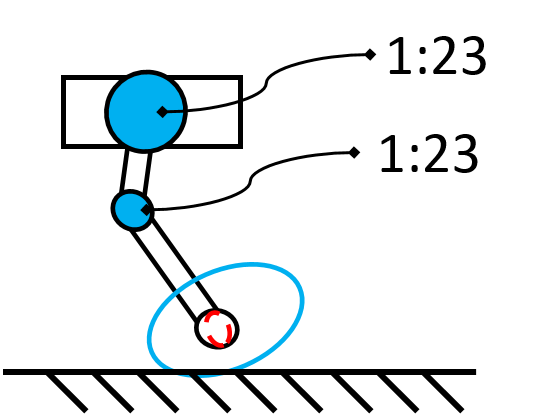
\includegraphics[width=0.35\textwidth]{legHS.png}
				\label{fig:legHS}}
        \subfloat[High load bearing]{
				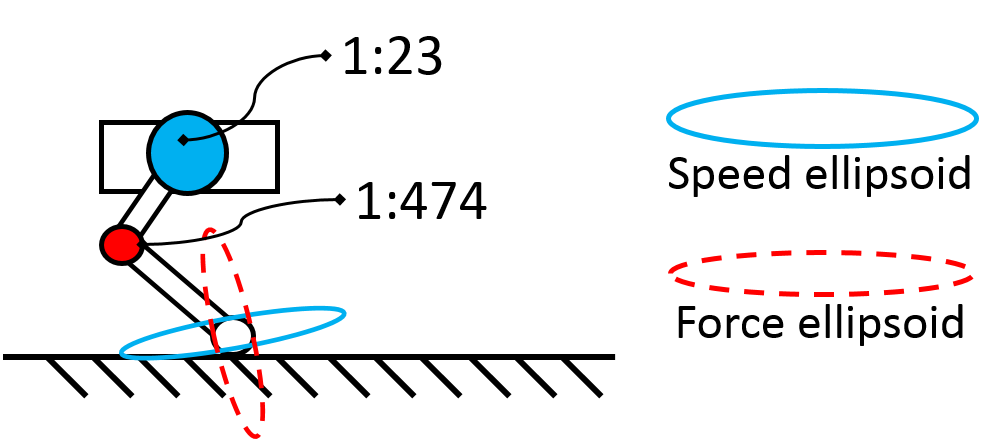
\includegraphics[width=0.65\textwidth]{legHF.png}
				\label{fig:legHF}}
        \caption{Advantageous gear-ratio selection for locomotion}\label{fig:legsol}
\end{figure}


\section{Experiments}
\label{sec:case_exp}



